This section is completely depended upon the hardware. It is composed of only hardware all combined together to form a suitable environment for brewing. All the hardware must be connected properly with the system to ensure quality beverages. 

\subsection{Layer Hardware}
The most important hardware required for this layer are three vessels/kettles, probably of 5 gallon each. Each vessel is connected to the 330 GPH Low Suction Electric pumps with suction hose to pump the liquid out of the vessels and DS18B20 Thermometer Temperature Sensor Probe in order to keep track of the temperature in each vessel.

\subsection{Layer Operating System}
There is no operating system involved in this layer. However, the temperature data and the pump of this layer is controlled by the Arduino Uno micro controller which is in different layer. 

\subsection{Layer Software Dependencies}
Since this is completely hardware dependent layer, there is no any software dependencies.
\newline

\begin{figure}[h!]
	\centering
	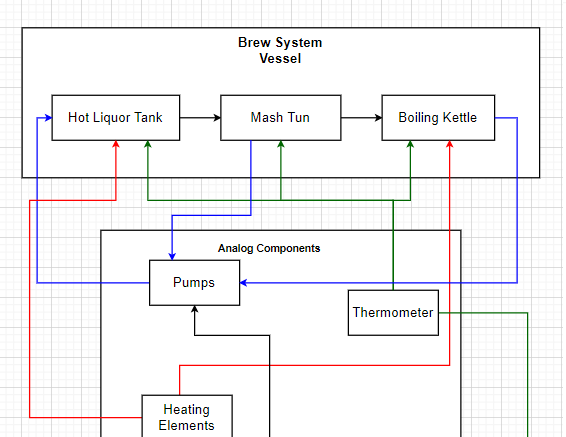
\includegraphics[width=0.60\textwidth]{images/Brew_System_Vessels}
	\caption{Brew System Vessel Layer Representation}
\end{figure}

\subsection{Hot Liquor Tank Subsystem (HLT)}
The main purpose of Hot Liquor Tank subsystem is to monitor and heat the water to the desired temperature. This subsystem is simply a vessel hardware used for boiling purpose.

\subsubsection{Subsystem Hardware}
Apart from the hardware mentioned above, this subsystem have one more hardware involved which is a Kettle Heating Element.

\subsubsection{Subsystem Operating System}
No Operating System is involved in this subsection.

\subsubsection{Subsystem Software Dependencies}
The Heating Element is depended on the input provided by the user on the basis of temperature as the water is only heated to that temperature. So, this subsystem require input from the user/brewer to properly function.

\subsubsection{Subsystem Programming Languages}
In order to provide the input, the user is using Arduino programming language for Arduino Uno.

\subsubsection{Subsystem Data Structures}
No specific data structures are being used in this subsystem. It is plain number being passed in and out of this subsystem.

\subsubsection{Subsystem Data Processing}
The thermometer temperature sensor probe reads the data and simply passes it to micro controller and the micro controller uses that data in order to raise the temperature of water by turning on or off the heating element. \newline

\subsection{Mash Tun Subsystem}
The main purpose of Mash Tun subsystem is to mix the hot water with grains to produce wort. This subsystem is simply a vessel hardware to separate mash and wort.

\subsubsection{Subsystem Hardware}
There are no separate hardware used in this subsystem.

\subsubsection{Subsystem Operating System}
No Operating System is involved in this subsection.

\subsubsection{Subsystem Software Dependencies}
The hardware used in this subsystem are not software dependencies.

\subsubsection{Subsystem Programming Languages}
No programming languages are used.

\subsubsection{Subsystem Data Structures}
No specific data structures are being used in this subsystem. there is just a float value being passed out of this subsystem.

\subsubsection{Subsystem Data Processing}
The thermometer temperature sensor probe reads the data and simply passes it to micro controller. \newline


\subsection{Boiling Kettle Subsystem}
The main purpose of Boiling Kettle subsystem is to boil wort for the required amount of time. This subsystem is simply the final vessel hardware used to produce beverage.

\subsubsection{Subsystem Hardware}
Apart from the hardware mentioned above, this subsystem have more hardware involved like a Kettle Heating Element and a NY Brew Supply copper wort chiller.

\subsubsection{Subsystem Operating System}
No Operating System is involved in this subsection.

\subsubsection{Subsystem Software Dependencies}
The software dependencies is similar to Hot Liquor Tank Subsystem. The Heating Element is depended on the input provided by the user on the basis of temperature as the wort is only heated to that temperature.

\subsubsection{Subsystem Programming Languages}
In order to provide the input, the user is using Arduino programming language for Arduino Uno.

\subsubsection{Subsystem Data Structures}
No specific data structures are being used in this subsystem. It is plain number being passed in and out of this subsystem.

\subsubsection{Subsystem Data Processing}
The thermometer temperature sensor probe reads the data and simply passes it to micro controller and the micro controller uses that data in order to raise the temperature of water by turning on or off the heating element. After the desired time is reached, the wort is sent to chiller which then cool downs to form beverages. \newline
